
\chapter{Rhythmic Similarity}\label{rhythmsimc}

This chapter provides an overview over some of the possibilities of computing music similarity by focusing on rhythmic features of different songs. \\
\textit{Tempo Estimation}

\section{Beat Histogram}

\textit{\textbf{Beat Histogram}}\\
Simple usage of beat histogram using euclidean distance \cite{rhythm1}. 

\begin{figure}[htbp]
	\centering
	\framebox{\parbox{1\textwidth}{
			\begin{subfigure}{.495\textwidth}
				\centering
				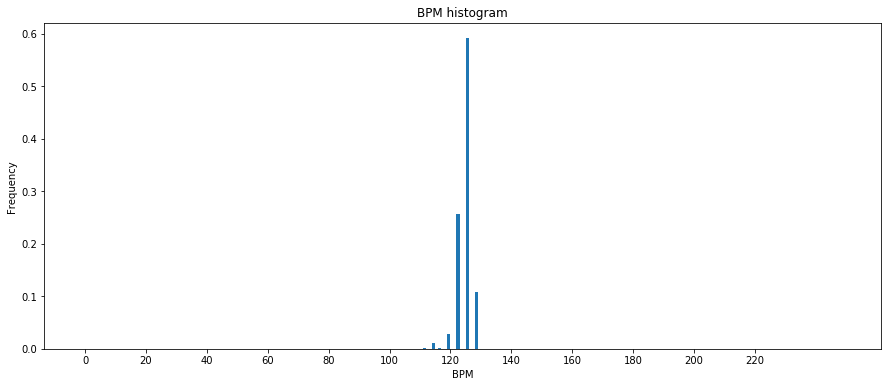
\includegraphics[scale=0.25]{Images/Beat/h_o_bh.png}
				\caption{Scorpions}
				\label{hobh}
			\end{subfigure}%
			\begin{subfigure}{.495\textwidth}
				\centering
				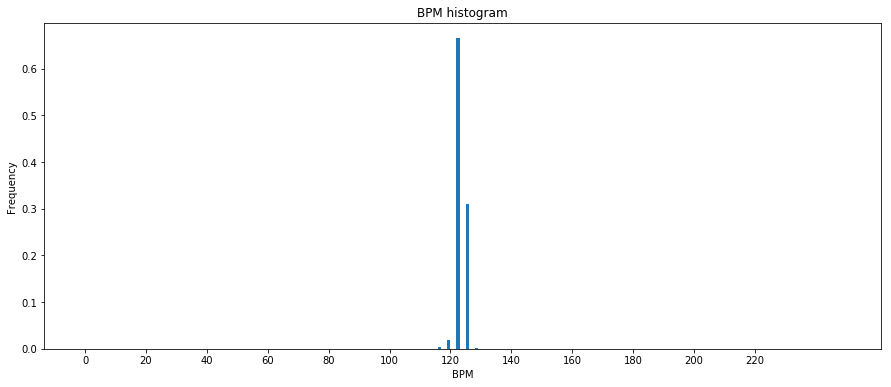
\includegraphics[scale=0.25]{Images/Beat/h_c_bh.png}
				\caption{Knightsbridge}
				\label{hcbh}
			\end{subfigure}% 
			
			\begin{subfigure}{.495\textwidth}
				\centering
				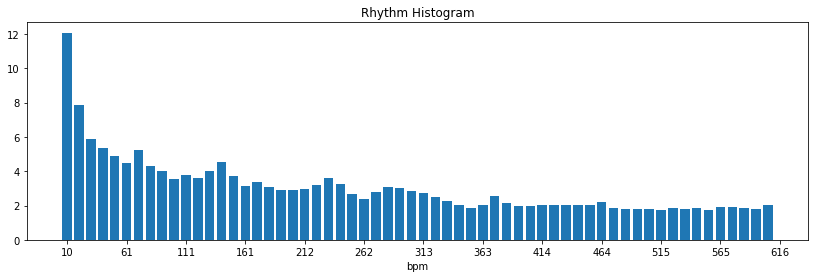
\includegraphics[scale=0.25]{Images/Beat/s_s_bh.png}
				\caption{94' Version Stanne}
				\label{ssbh}
			\end{subfigure}%
			\begin{subfigure}{.495\textwidth}
				\centering
				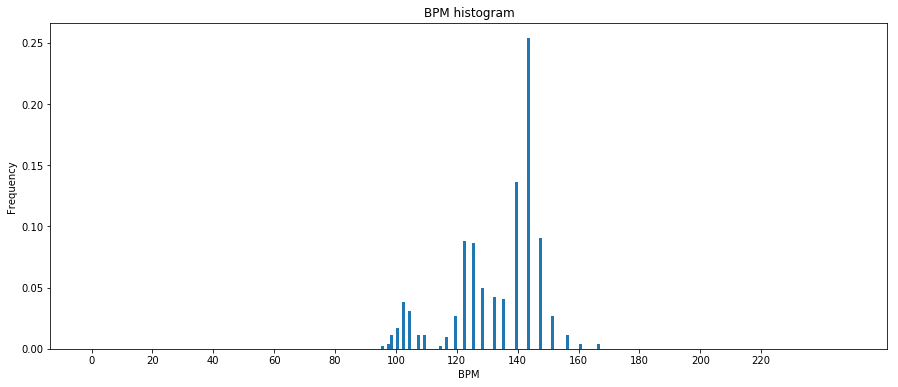
\includegraphics[scale=0.25]{Images/Beat/s_a_bh.png}
				\caption{99' Version Stanne}
				\label{sabh}
			\end{subfigure}%			
	}}
	\caption{Beat Histogram}
	\label{fig:bh1}
\end{figure}

Gruhne (et al.) suggests an additional post processing step for the beat histogram. They found, that logarithmic re-sampling of the lag axis of the histogram and cross-correlation with an artificial rhythmic grid improves the performance of the similarity measurement further \cite[182]{rbh1}. 

\section{Rhythm patterns}

\textit{\textbf{Fluctuation Pattern, Onset Patterns, Rhythm Pattern}}\\
Using: rp\_extractor library from TU Vienna \cite{rp_extract}, Paper: \cite{rp1}, \cite{rp2}

\begin{figure}[htbp]
	\centering
	\framebox{\parbox{1\textwidth}{
			\begin{subfigure}{.495\textwidth}
				\centering
				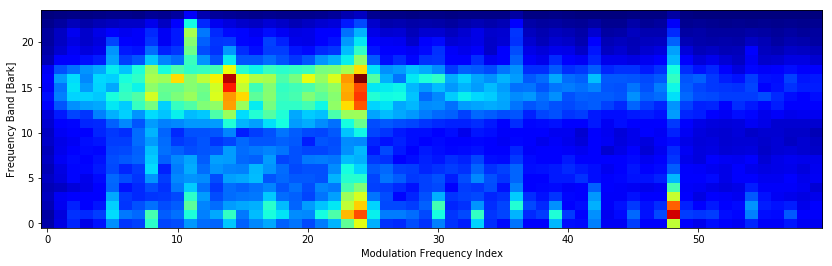
\includegraphics[scale=0.25]{Images/Beat/h_o_rp.png}
				\caption{Scorpions}
				\label{horp}
			\end{subfigure}%
			\begin{subfigure}{.495\textwidth}
				\centering
				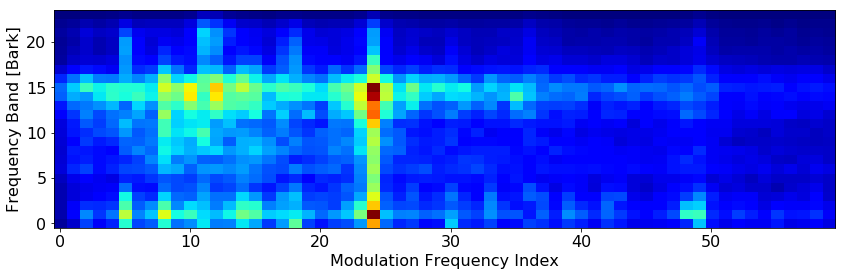
\includegraphics[scale=0.25]{Images/Beat/h_c_rp.png}
				\caption{Knightsbridge}
				\label{hcrp}
			\end{subfigure}% 
			
			\begin{subfigure}{.495\textwidth}
				\centering
				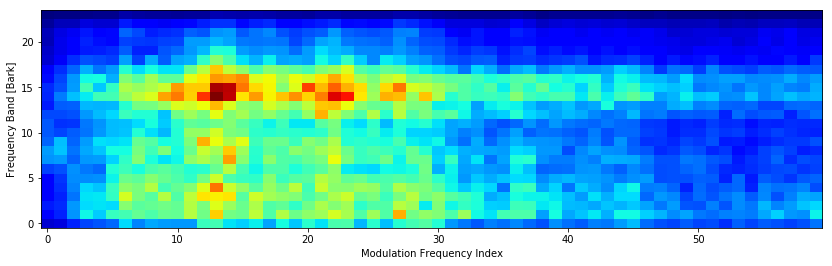
\includegraphics[scale=0.25]{Images/Beat/s_s_rp.png}
				\caption{94' Version Stanne}
				\label{ssrp}
			\end{subfigure}%
			\begin{subfigure}{.495\textwidth}
				\centering
				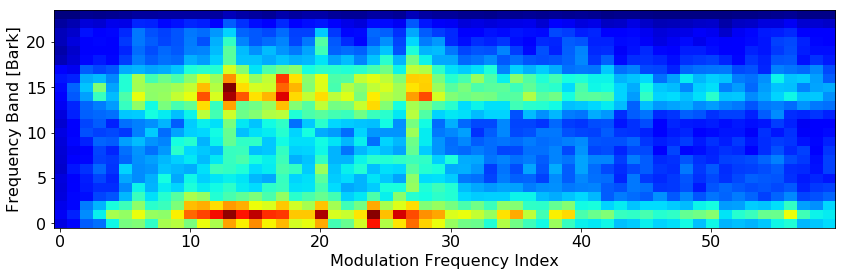
\includegraphics[scale=0.25]{Images/Beat/s_a_rp.png}
				\caption{99' Version Stanne}
				\label{sarp}
			\end{subfigure}%			
	}}
	\caption{Rhythmic Patterns}
	\label{fig:rp1}
\end{figure}

\section{Cross Correlation}

\textit{\textbf{Onset signal}}\\

- simple approach using only onset and beat features extracted with librosa
- cross correlation of 2 songs

dependent on beat extraction and onset detection algorithms

\begin{figure}[htbp]
	\centering
	\framebox{\parbox{1\textwidth}{ 			
			\begin{subfigure}{.495\textwidth}
				\centering    
				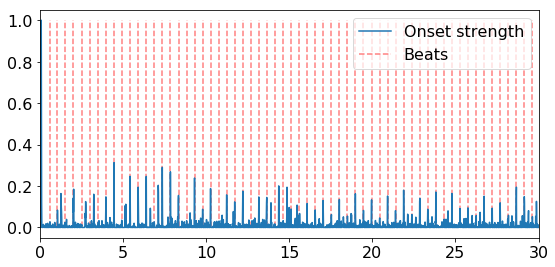
\includegraphics[scale=0.3]{Images/Beat/h_o_on.png}
				\caption{Scorpions}
				\label{hoon}
			\end{subfigure}		
			\begin{subfigure}{.495\textwidth}
				\centering     
				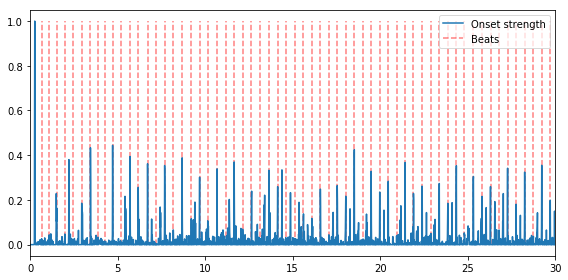
\includegraphics[scale=0.3]{Images/Beat/h_c_on.png}
				\caption{Knightsbridge}
				\label{hcon}
			\end{subfigure}%			
	}}
	\caption{Detected Onsets (first 30 seconds)}
	\label{fig:ons1}
\end{figure}	